\chapter{Datenerhebung von GitHub Projekten} \label{kap:Datenerhebung}

% Ziel der Datenerhebung
Das Ziel dieser Datenerhebung ist es die Hypothesen H1, H2, H4, H5, und H8 zu prüfen.
Hier wurden 108 Open Source Projekte auf GitHub ausgewählt.
% Rahmenbedingungen
Die Studie von Midha et al. hat sich auf die Programmiersprachen C++ beschränkt, ähnlich wird sich
auch diese Arbeit auf JavaScript (JS) und TypeScript (TS) beschränken. Grund hierfür ist, dass
sich verschiedene Programmiersprachen schlecht miteinander vergleichen lassen
\cite{midhaFactorsAffectingSuccess2012}.
JavaScript wurde für die Datenerfassung ausgewählt, da es zurzeit die Sprache mit den meisten
Projekten auf GitHub ist.
% Why TypeScript? What is TypeScript? 
TS wird mit aufgenommen, da es ein Obermenge von JS ist. TypeScript kann in JS-Scripten verwendet
werden, dies hätte zur Folge, dass diese als JavaScript kennzeichnen. Aus diesem Grund wird TS explizit
mit in die Datenerhebung mit aufgenommen.

Erhoben wurden nur Software-Projekte. Repositories wie E-Books, Tutorials oder Lehrplattformen wurden
ausgeschlossen. Projekt Archive wurden ebenfalls ausgeschlossen




% ------------------------------------------------------------------------------------------------ %
%                                     Manuelle Datenerfassung                                      %
% ------------------------------------------------------------------------------------------------ %
\section{Manuelle Datenerfassung}\label{sec:manuelle_datenerfassung}

% Wie wurden die Daten erfasst
Mithilfe der GitHub Suchfunktion\footnote{\url{https://github.com/search/advanced}} wurden JS und
TS Projekte ausgewählt. Die Ausgabe wurde nach Anzahl Sternen sortiert wiedergegeben und in
dieser Reihenfolge erfasst.
% None MIT-Search
Die Ausgabe der ersten Suche beinhaltete überwiegende Mehrzahl der Projekte mit MIT Lizenz. Um eine
höhere Diversität des Lizenzen-Milieus zu gewährleisten, wurde im Laufe der Datenerfassung explizit,
nach nicht MIT lizenzierten Projekten gefiltert.
% Was wurde erfasst [pt. 1]
Zum Erfassen der Daten wurde ein selbst entwickeltes Web-Interface verwendet, um die Erhebung
zu vereinfachen. Wie in Abbildung \ref{abb:Web_Interface} zu sehen ist wurden zunächst
Identifikationsdaten notiert. Für GitHub wurde \textit{<owner>/<project>} verwendet,
wie sie auch in der URL oder auf der Project Page zu finden sind. Für NPM wurde der Package Name
verwendet, falls dieser vorhanden war. Applikationen beispielsweise haben in den meisten
Fällen kein NPM Package.
% Was wurde erfasst [pt. 2]
Des Weiteren wurden auch Niveau der Dokumentation, Vorhandensein von Sponsoren, wer hinter dem
Projekt steht und um was für ein Typ Projekt es sich handelt gesammelt.
% Einführung nächste Kapitel
Alle Einträge wurden an ein NodeJS Backend gesendet und als CSV abgespeichert.
Im den nächsten Unterkapiteln wird näher erläutert, wie die Kriterien, die von Hand erfasst wurden,
zustande gekommen sind und welche Bedeutung die Werte in der CSV-Datei haben.

% ----------------------------------- Abbildung: Web Interface ----------------------------------- %
\newpage %! new page
\begin{figure}[h]
    \centering
    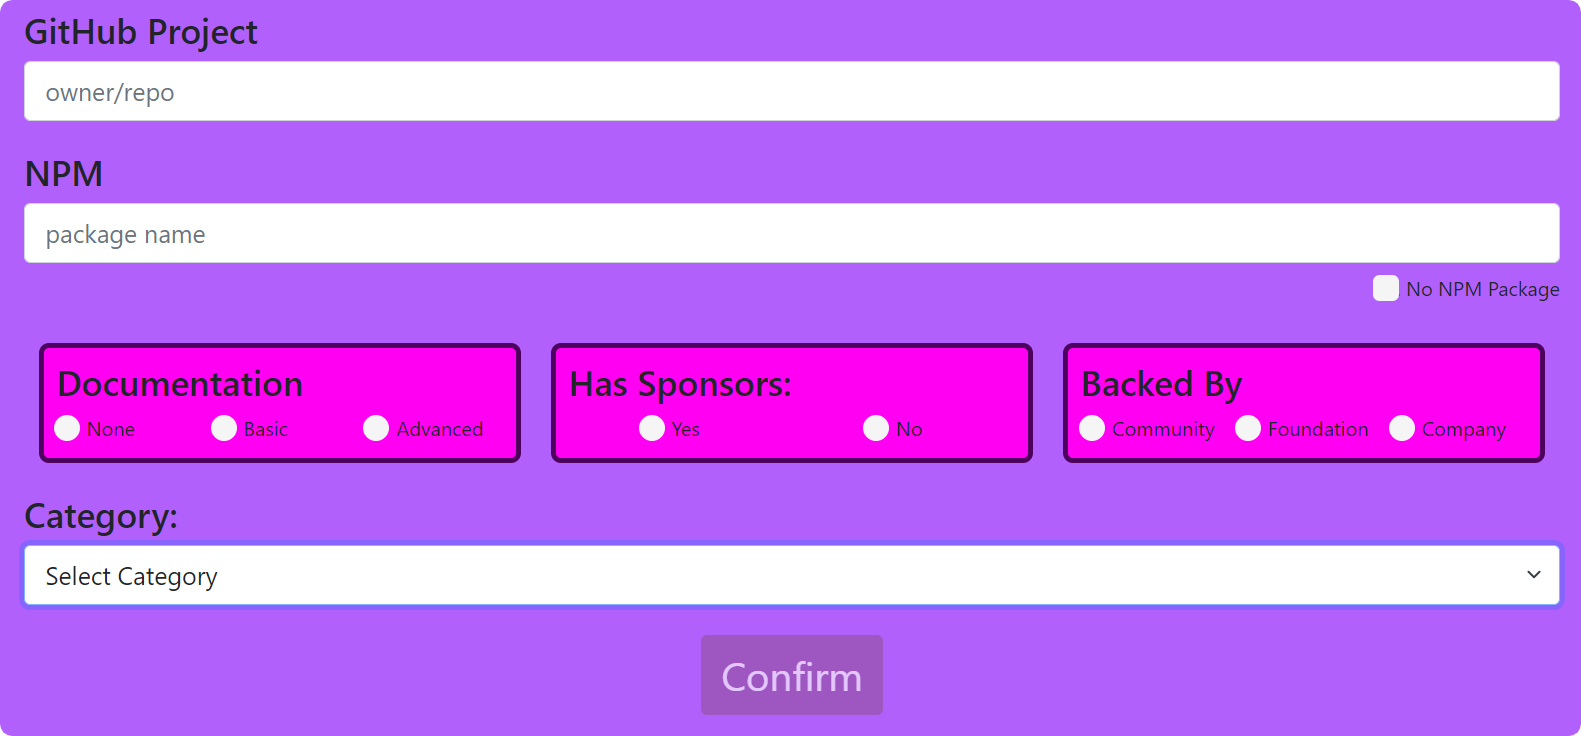
\includegraphics[scale=0.25]{figures/04/WebInterface.png}
    \caption{Web-Interface}
    \label{abb:Web_Interface}
\end{figure}



% ----------------------------------------- Dokumentation ---------------------------------------- %
\subsection{Dokumentation} \label{ssec:manuelle_datenerfassung_dokumentation}
Die Dokumentation des Projektes wurde analysiert und nachfolgenden Kriterien kategorisiert:

\begin{itemize}[noitemsep]
    \item[0 =] keine Dokumentation
    \item[1 =] basis Dokumentation, rein textuell
    \item[2 =] Dokumentationen mit Demos oder Live-Beispielen,
        Einführungsvideos oder ähnliches
\end{itemize}


% ------------------------------------------- Sponsoren ------------------------------------------ %
\subsection{Sponsoren}
Für jedes Projekt wurde geprüft, ob es Sponsoren hat. Die Anzahl an Sponsoren bzw. die Einnahmen
durch Sponsoren wurden nicht beachtet. Das Vorhandensein der Sponsoren wurde wie folgt codiert:

\begin{itemize}[noitemsep]
    \item[0 =] hat keine Sponsoren
    \item[1 =] hat Sponsoren
\end{itemize}


% ------------------------------------------- Backed by ------------------------------------------ %
\subsection{Backed By} % TODO KAPITEL UMBENNENEN


Im nächsten Schritt wurde vermerkt wer hinter einem Projekt steht, hierbei wurde in drei Kategorien
eingeteilt:

\begin{itemize}[noitemsep]
    \item[0 =] Eines reinen Community Projektes unabhängig von Unternehmen. Beispiel: VueJS.
    \item[1 =] Von einer Stiftung wie OpenJS\footnote{\url{https://openjsf.org/}} unterstütztes oder
        entwickeltes Projekt.\\ Beispiel: NodeJS.
    \item[2 =] Projekte die von Unternehmen entwickelt werden, wie React von Facebook beispielsweise.
\end{itemize}

\noindent
Diese Information fanden sich entweder auf der GitHub-Page, Homepage des Projektes oder das Unternehmen
ist der Besitzer des Repositories.



% ------------------------------------------- Kategorie ------------------------------------------ %
\newpage %! NewPage
\subsection{Projektarten}
Im letzten Schritt wurde das Projekt in eins der folgenden Kategorien zugeordnet:

\begin{multicols}{2}
    \begin{itemize}
        \setlength\itemsep{0em}
        \item Utility
        \item UI
        \item Application
        \item Library
        \item Framework
        \item Test-Framework
        \item Open-Core
        \item API
    \end{itemize}
\end{multicols}

% Erläuterung der Kategorien
\subsubsection*{Erläuterung der Kategorien}

\begin{itemize}
    \setlength\itemsep{0em}
    \item \textbf{Utility}, wurden Projekte kategorisiert, die nicht direkt in Projekte eingebaut
          werden, sondern als Tool verwendet werden. Beispiel: \texttt{shelljs/shelljs}\footnote{
              \url{https://github.com/shelljs/shelljs}}
    \item \textbf{Application}, sind eigenständige Produkte wie draw.io\footnote{
              \url{https://github.com/jgraph/drawio}}
\end{itemize}





% ------------------------------------------------------------------------------------------------ %
%                                                                                                  %
%                                   Automatisierte Datenerfassung                                  %
%                                                                                                  %
% ------------------------------------------------------------------------------------------------ %
\newpage %! newpage
\section{Automatisierte Datenerfassung}\label{sec:automatisierte_datenerfassung}

Im zweiten Teil der Erhebung wurden weitere Daten automatisiert gesammelt. Hierfür wurde die
GitHub API\footnote{\url{https://docs.github.com/en/rest}}, NPM
API\footnote{\url{https://github.com/npm/registry}} und für einige Daten Web-Scraping
verwendet.

Zu diesem Zweck wurde eine weitere NodeJS Applikation geschrieben, welche die CSV-Datei aus dem
Kapitel \ref{sec:manuelle_datenerfassung} ausliest und mithilfe der APIs und Web-Scraping eine neue
CSV-Datei generiert. In Abbildung \ref{abb:Architektur} wird der Prozess der Datenerhebung grafisch
dargestellt. In den folgenden Unterkapiteln wird aufgelistet welche Daten mittels welcher Methode gesammelt wurden.


% ----------------------------------- Daten aus der GitHub API ----------------------------------- %
\subsection{Daten aus der GitHub API}
Mittels der GitHub API wurden folgende Daten gesammelt:

\begin{itemize}[noitemsep]
    \item Anzahl der GitHub-Sternen
    \item Erstellungsdatum des Repositories
    \item Vorhandensein einer \textit{CODE\_OF\_CONDUCT.md}
    \item Vorhandensein einer \textit{CONTRIBUTING.md}
    \item Lizenz
    \item Anzahl der Commits in den letzten 12 Monaten
    \item Anzahl der Issues in den letzten 12 Monaten
\end{itemize}

% * GitHub_generalInfo
% * projectHealth
% * commitActivity
% * issues_PRs

% ------------------------------------- Daten aus der NPM API ------------------------------------ %
\subsection{Daten aus der NPM API}
Mit der NPM API wurden die Downloads der letzten 7 Tage abgefragt.

% * npm_downloads

% ---------------------------------- Daten aus dem Web-Scraping ---------------------------------- %
\subsection{Daten aus dem Web-Scraping}
Mithilfe von Web-Scraping wurden folgende Daten erfasst:

\begin{itemize}[noitemsep]
    \item Die Anzahl von \textit{UsedBy} auf der GitHub Page des Projektes.
    \item Anzahl der Gesamt-Commits auf dem default Branch
    \item Anzahl der Mitwirkenden
\end{itemize}

\subsubsection*{Anmerkung:}
Ein Mitwirkender zählt nur dann als solcher, wenn dessen Commit entweder auf dem \textit{default}
oder \textit{gh-pages} Branch liegt. Die Commits auf anderen Branches werden nur dann gezählt,
wenn ein merge auf einen der vorherig erwähnten Branches stattfindet. Gleiches gilt für Commits \cite{GHapiDocsCommits}.

% * GitHub_usedBy
% * GitHub_Page
% * npm_dependants


% ----------------------------------- Nachbearbeitung der Daten ---------------------------------- %
\subsection{Nachbearbeitung der Daten}

Nachdem erheben der Daten war eine Nachbearbeitung notwendig. Einige Projekte hatten die Lizenz
\texttt{other}. Der Grund hierfür ist, dass die \texttt{LICENSE.md} nicht dem Standardtext einer
Lizenz entsprochen hat. Ein Beispiel wäre die Lizenz von
meteor\footnote{\url{https://github.com/meteor/meteor/blob/devel/LICENSE}},
welche nach dem offiziellen Lizenztext noch eine Anmerkung bezüglich benutzter Bibliotheken hat.
Alle als \texttt{other} gekennzeichneten Projekte wurden manuell geprüft und korrigiert.
%
Zudem wurden Projekte ohne Lizenzen oder Lizenzen die nicht von der \textit{Open Source Initiative}
zugelassene sind komplett aussortiert.
%
Nach dem gleichen Prinzip wurden Projekte kontrolliert, die laut API kein Contributing Guide bzw. kein Code
of Conduct haben. Grund hierfür ist, dass GitHub das Vorhandensein dieser Dateien nur dann erkennt,
wenn diese im Hauptverzeichnis liegen und exakt \texttt{CONTRIBUTING.md} bzw \texttt{CODE\_OF\_CONDUCT.md}
heißen. Einige Projekte hatten Tippfehler in den Dateinamen, oder den Contributing Guide bzw Code of Conduct
war Teil der README.md statt eine eigene Datei bzw. auf der Website des Projektes.
% 9 Datensätze wurden korrigiert (Contributing) / 2 Datensätze wurden bezüglich (CoC) korrigiert





% ------------------------------------ Abbildung: Architektur ------------------------------------ %
\begin{figure}[h]
    \centering
    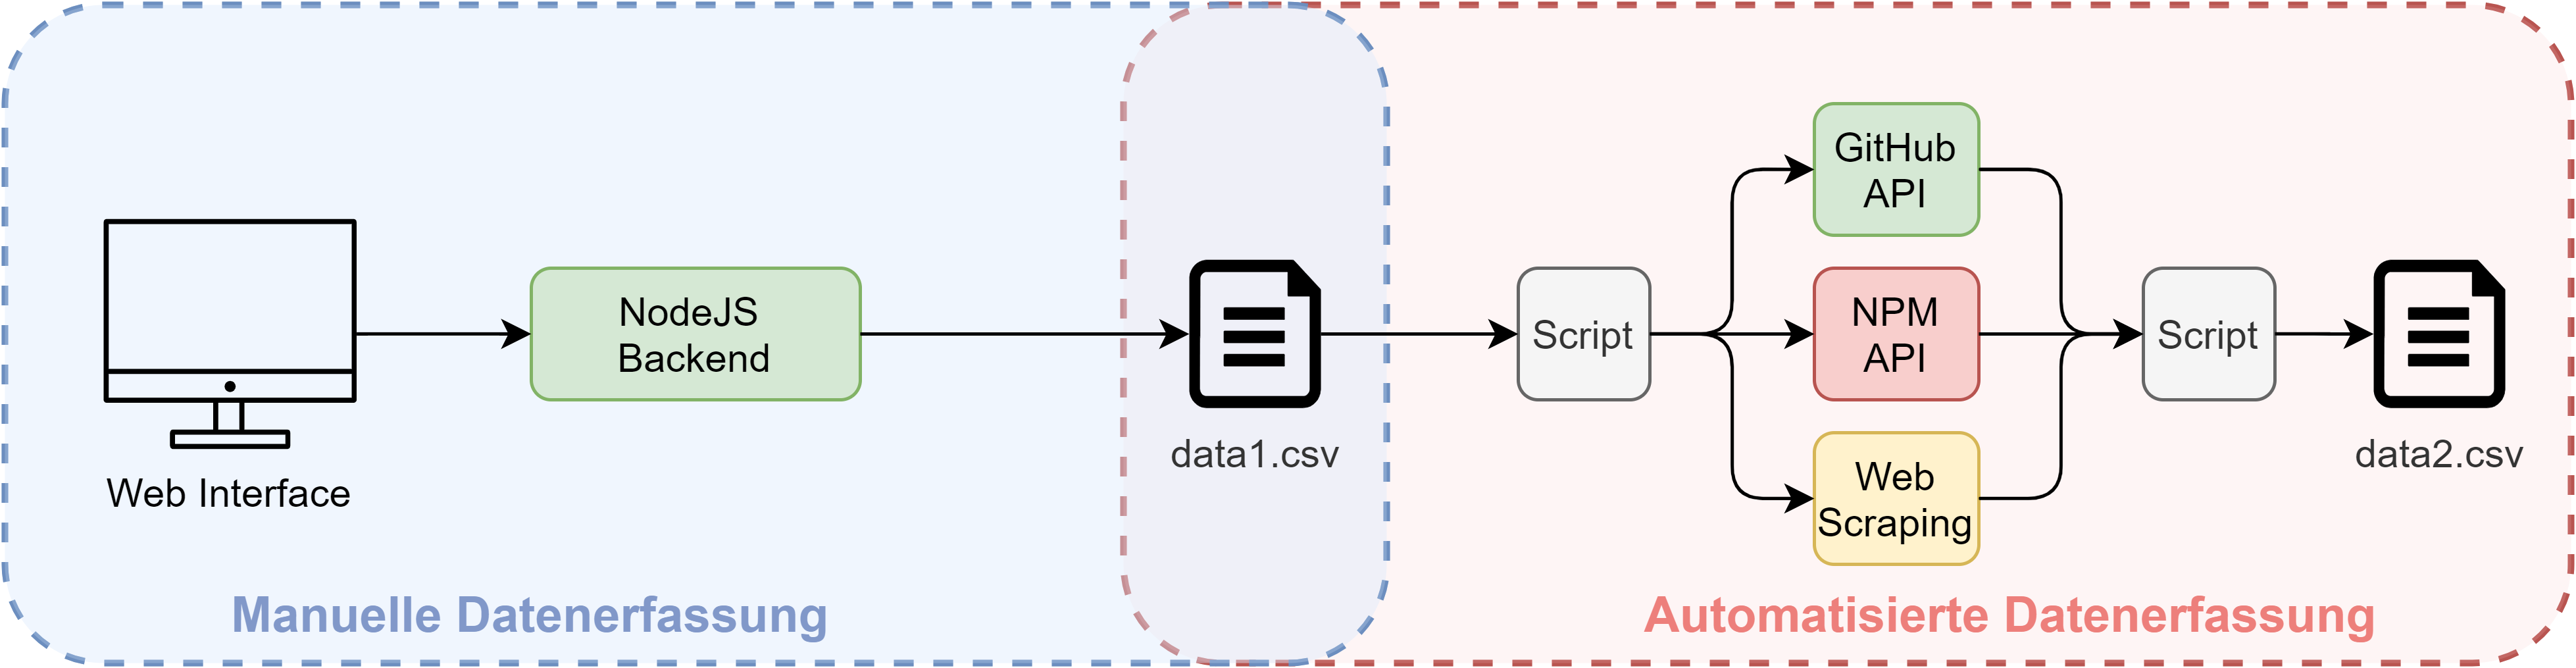
\includegraphics[scale=0.1]{figures/04/DatenerfassungArchitektur.png}
    \caption{Prozess der Datenerhebung}
    \label{abb:Architektur}
\end{figure}


% \section{Top 100 Projekte}\label{sec:top_100_projects}

% \xodoo{Datenerhebubg der Top 100 Projekte, unabhängig von Programmiersprache. Ziel: Besseren eindruck
% über Lizenzen. Vorgehen: Wie zuvor auch, keine Tutorials etc. Abgespeckte Version weil die meisten
% "Funktionen" des Haversters abgeschaltet wurdens sind.}

% Hier wird die Regel "Nur JS" gebrochen, da das Ziel ist GH-Sterne in Relation zu den Lizenzen zu 
% vergleichen.